\chapter{Тестовые расчеты} \label{ch:ch3}

В соответствии с~описанными математическими моделями были проведены расчеты нескольких тестовых задач. Значения параметров фаз и среды при расчетах указаны в таблицах~\ref{tabular:liquids},~\ref{tabular:medium}.

\begin{table}[!ht]
\captionof{table}{Параметры фаз}
\centering
\begin{tabular}{|c|c|c|c|}
\hline
Физ. величина & вода, \textit {w} & нефть, \textit {n} & газ, \textit {g} \\
\hline
Плотность,  $ {\text{кг}} / {\text{м}^3} $ & 1000 & 850 & 1.4 \\
\hline
Динамическая вязкость, $ \text{Па} \cdot \text{с} $ & $10^{-3}$ & $10^{-2}$ & $10^{-5}$ \\
\hline
Сжимаемость, $ \text{Па}^{-1}$ & $4.4 \cdot 10^{-10}$ & $10^{-9}$ & $10^{-5}$ \\
\hline
Остаточная насыщенность & 0.05 & 0.05 & 0.05 \\
\hline
\end{tabular}
\label{tabular:liquids}
\end{table}

\begin{table}[!ht]
\captionof{table}{Параметры среды}
\centering
\begin{tabular}{|c|c|}
\hline
Пористость & 0.4\\
\hline
Абсолютная проницаемость, $ \text{м}^{2}$ & $6.64 \cdot 10^{-11}$ \\
\hline
\end{tabular}
\label{tabular:medium}
\end{table}

\section{Одномерная двухфазная задача просачивания} \label{ch:ch3/sect1}

Для верификации и сравнения двух предложенных подходов к
моделированию фильтрации решим задачу о двухфазном течении воды и нефти
в однородной изотропной пористой среде в случае, когда имеет место накачка воды на границе.
Для более ощутимого влияния капиллярных сил, значение давления уменьшено.
Исследуемая область представляет собой параллелепипед размера 1м$\times$1м$\times$5м.
Задача сводится к одномерной по оси Oz (вдоль которой действует
сила тяжести) в силу симметрии. Постановка задачи изображена на~\ref{t1_pic1}.
Начальные условия: $S_w = 0.35$, $P_{avg} = 1.5 - 0.1z$.
Граничные условия: $\left.S_w\right|_{z = 0} = 0.7$, $\left.S_w\right|_{z = 5} = 0.35$, 
$\left.P_{avg}\right|_{z = 0} = 1.5 \text{атм}$, $\left.P_{avg}\right|_{z = 5} = 1 \text{атм}$.

Сравнение профилей водонасыщенности и среднего давления на момент времени 300 с при решении
тестовой задачи тремя различными методами проиллюстрировано на~\ref{t1_pic2}.
Method1 обозначает подход, основанный на гиперболической КГД
модели. Method2 - подход, учитывающий релаксацию потока. IMPES method представляет собой эталонное решение. В целом наблюдается согласование результатов.
Визуально результаты по методам II и IMPES совпадают в силу малости относительных ошибок. Результаты по методу I визуально близки к эталонному.

\begin{figure}
\centering
    \begin{minipage}[h]{0.49\textwidth}
       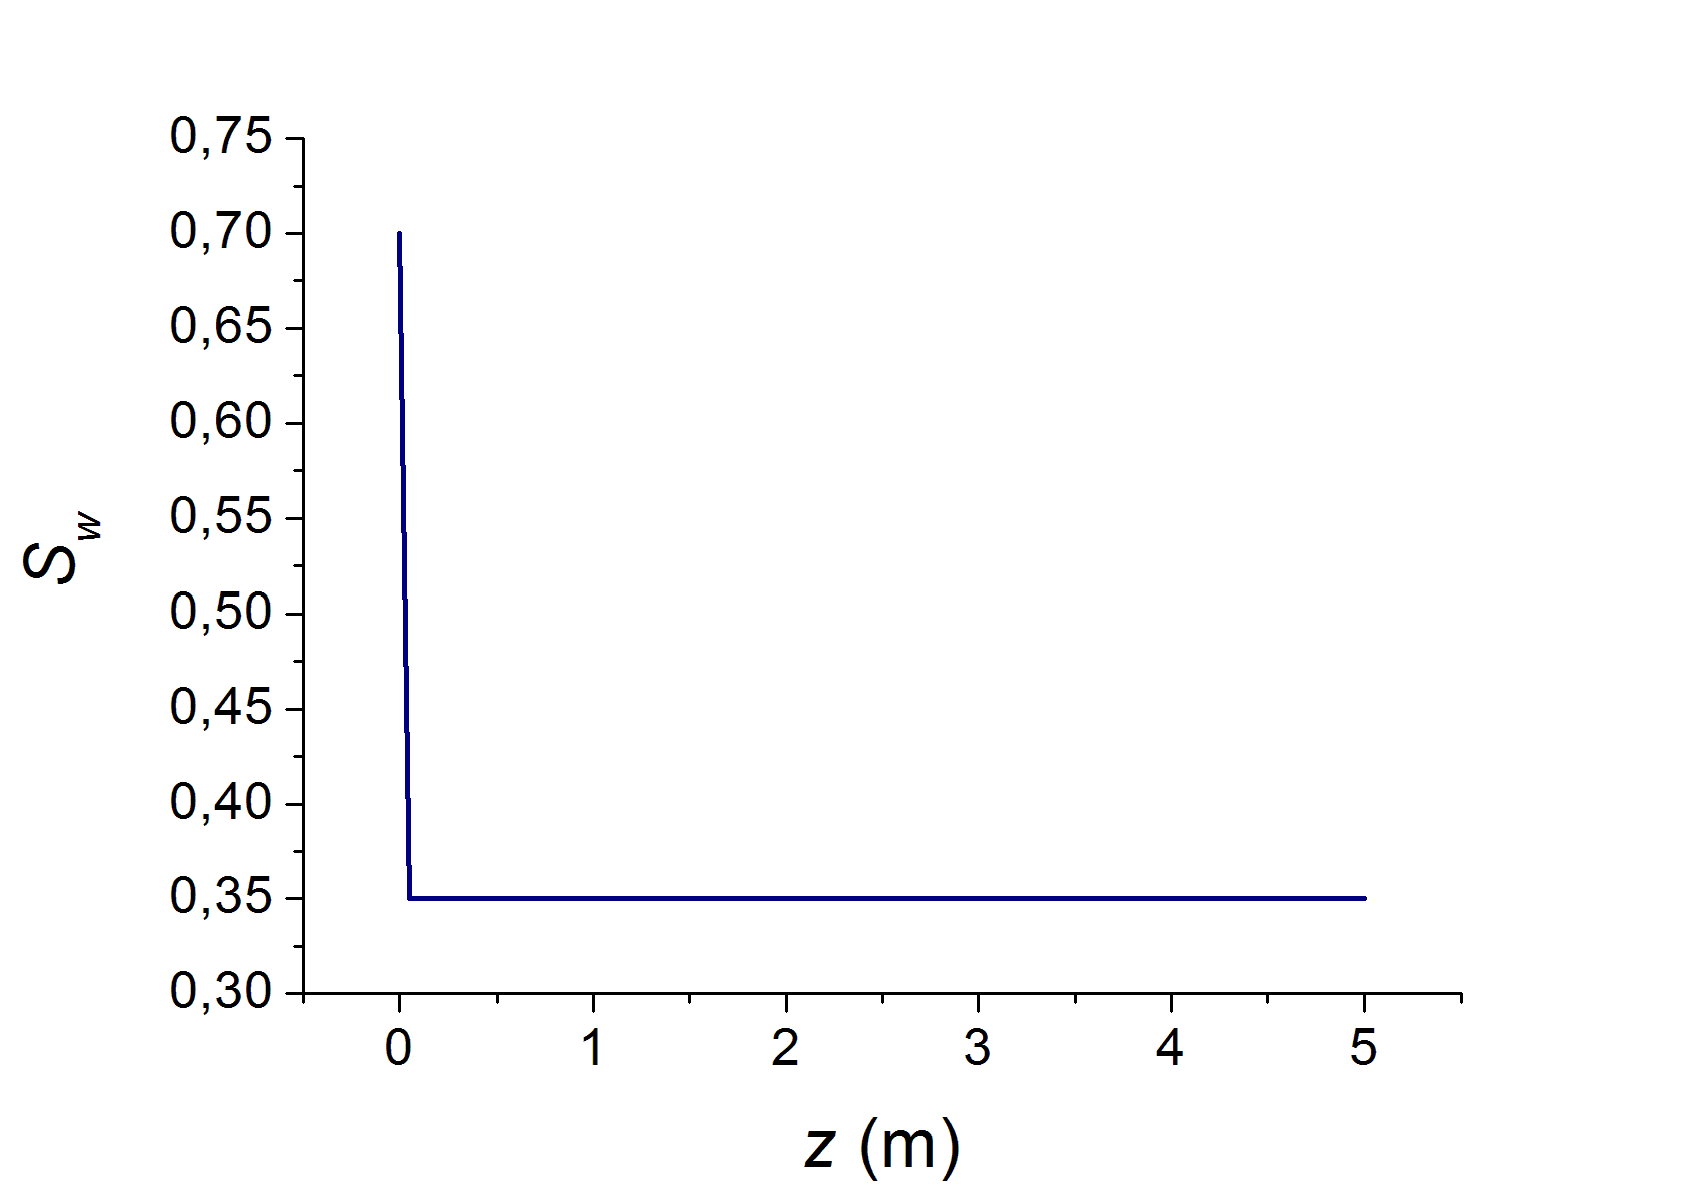
\includegraphics[width=1\textwidth]{test1/init1.png}
       \caption*{Водонасыщенность}
    \end{minipage}
    \hfill
    \begin{minipage}[h]{0.49\textwidth}
       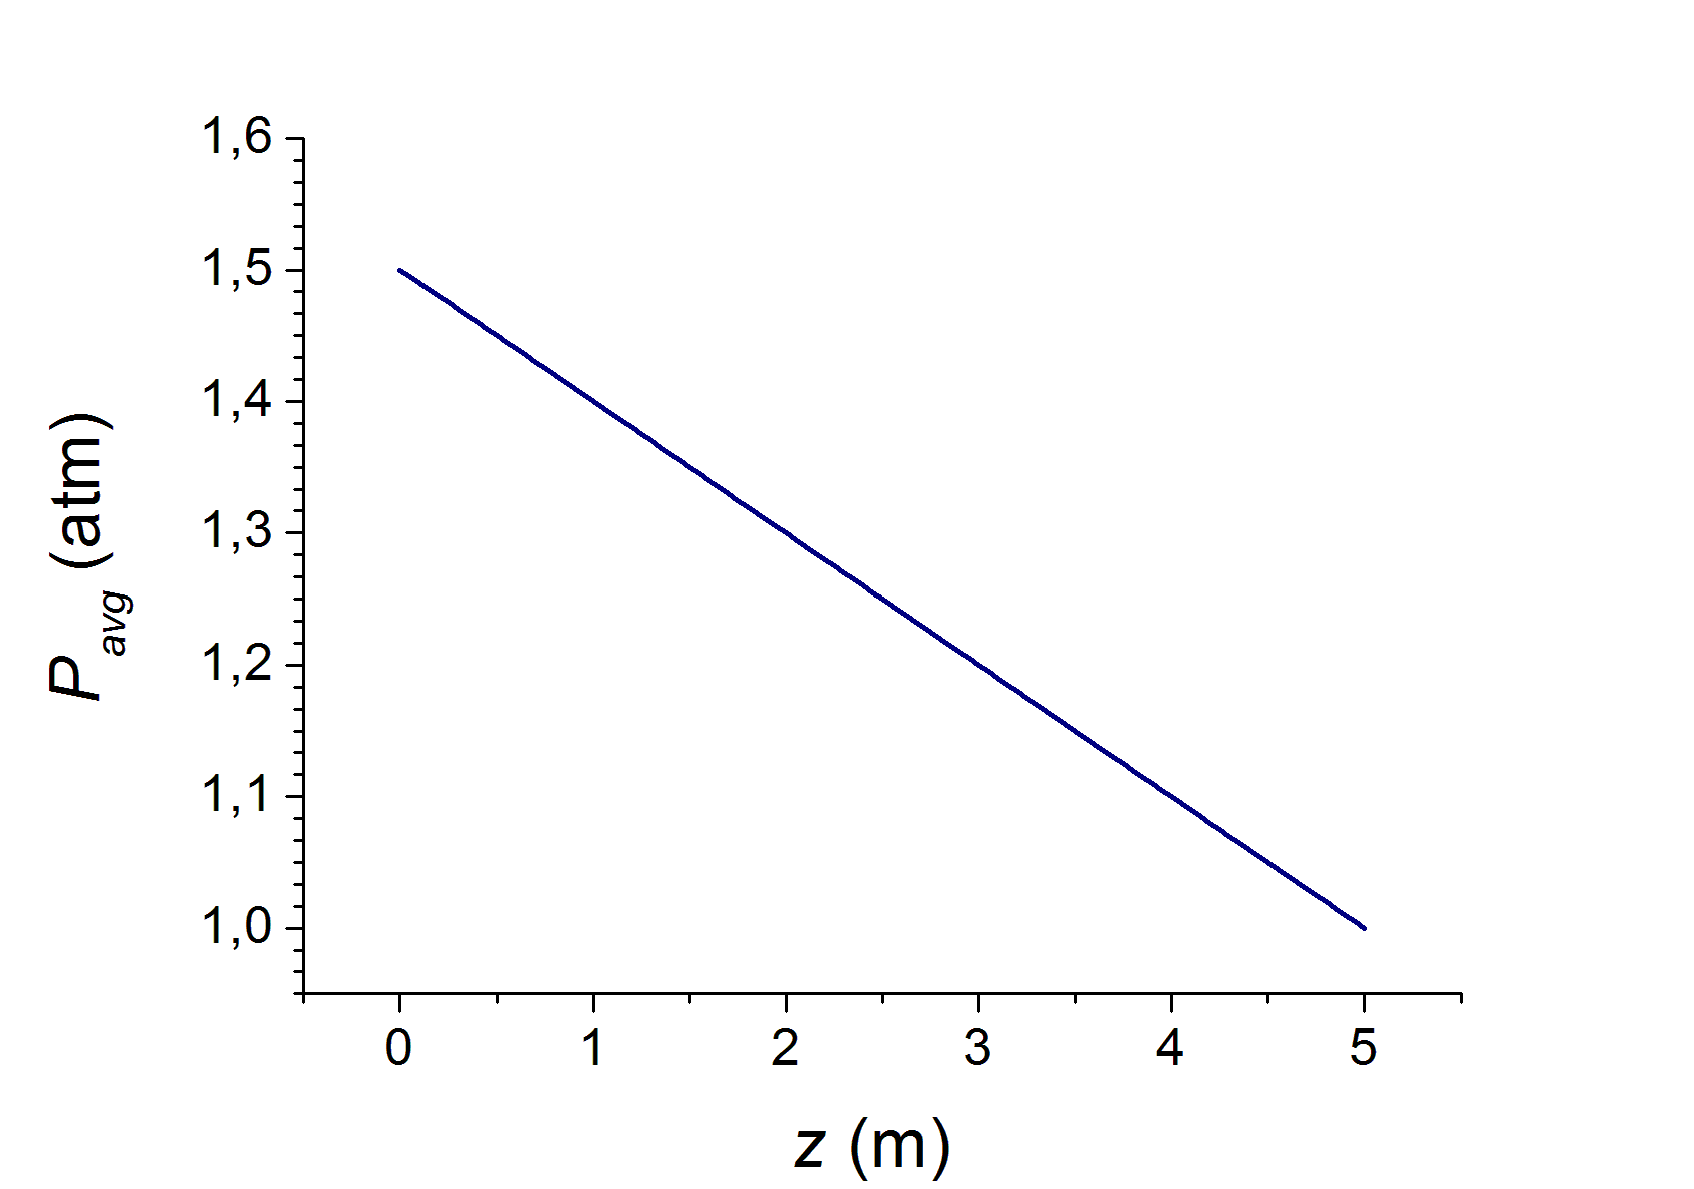
\includegraphics[width=1\textwidth]{test1/init2.png}
       \caption*{Среднее давление}
    \end{minipage}
  \caption{Распределение водонасыщенности и среднего давления фаз по глубине в начальный момент времени}
  \label{t1_pic1}
\end{figure}

\begin{figure}
\centering
    \begin{minipage}[h]{0.49\textwidth}
       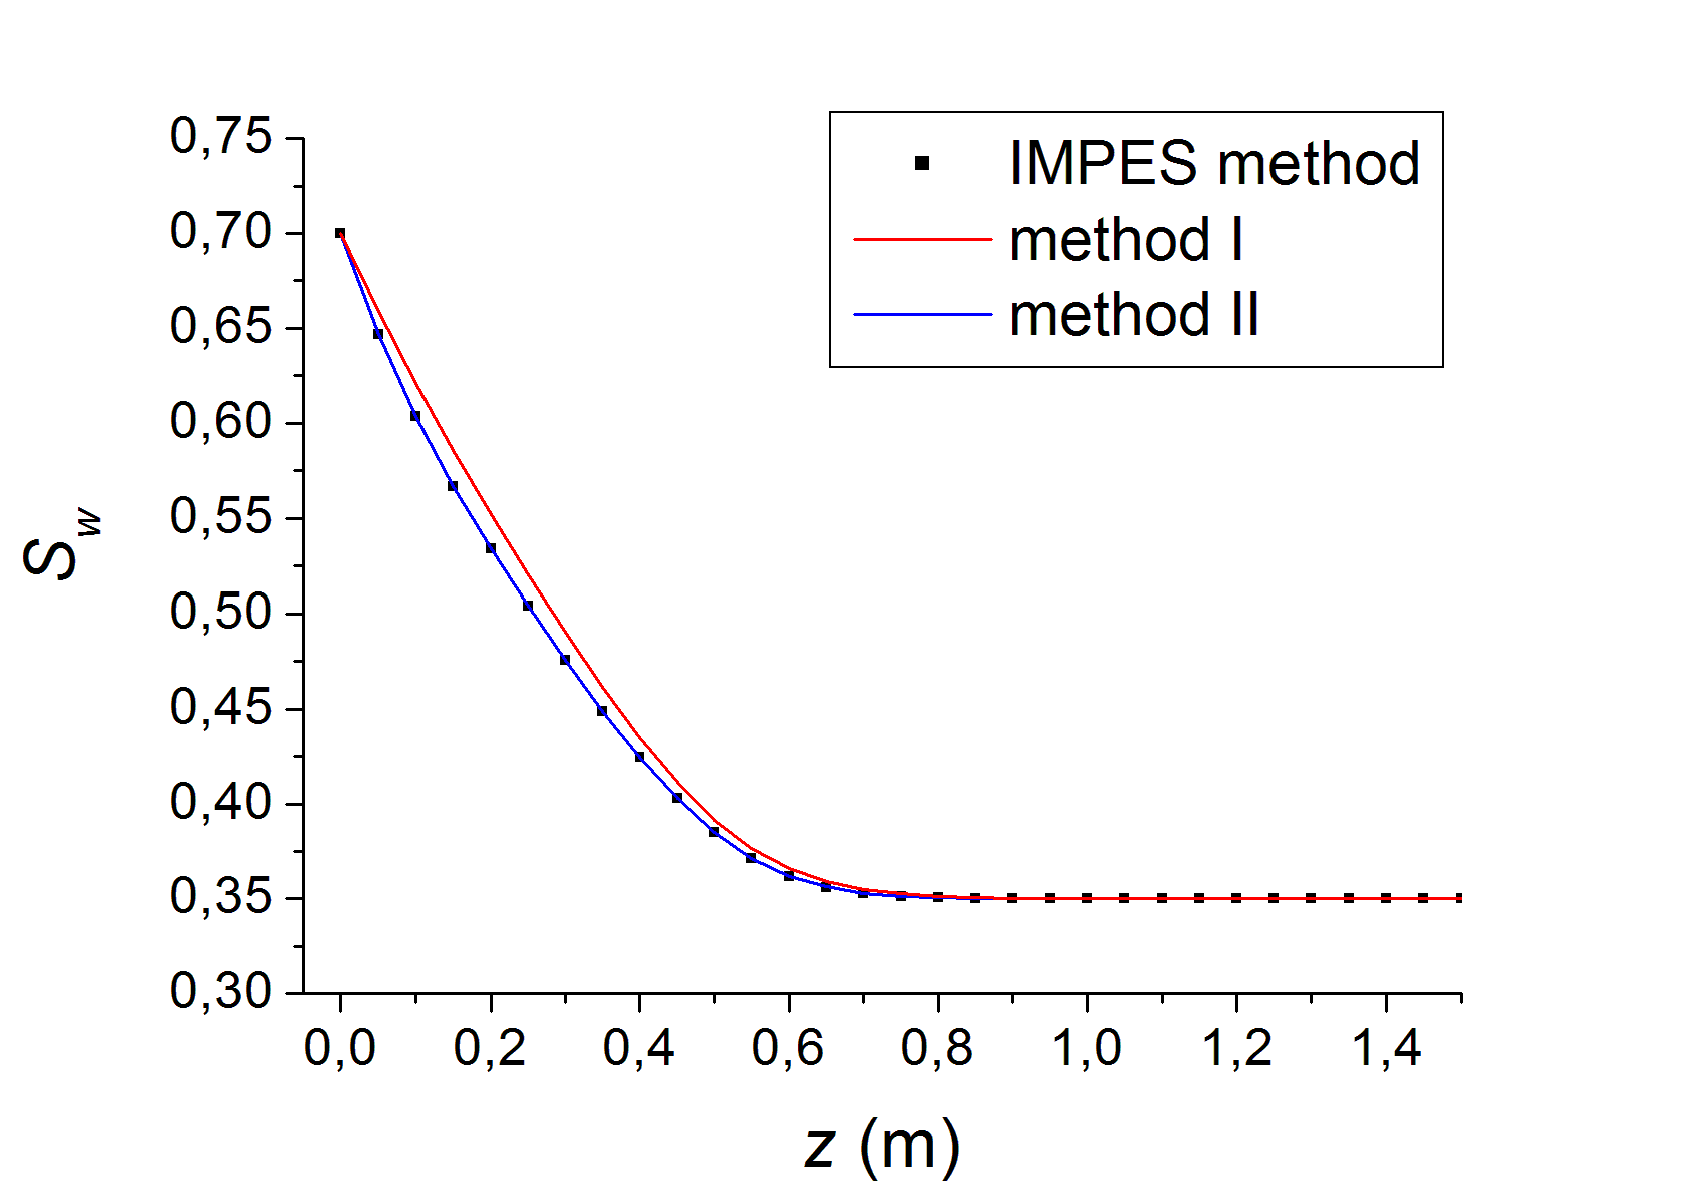
\includegraphics[width=1\textwidth]{test1/res1.png}
       \caption*{Водонасыщенность}
    \end{minipage}
    \hfill
    \begin{minipage}[h]{0.49\textwidth}
       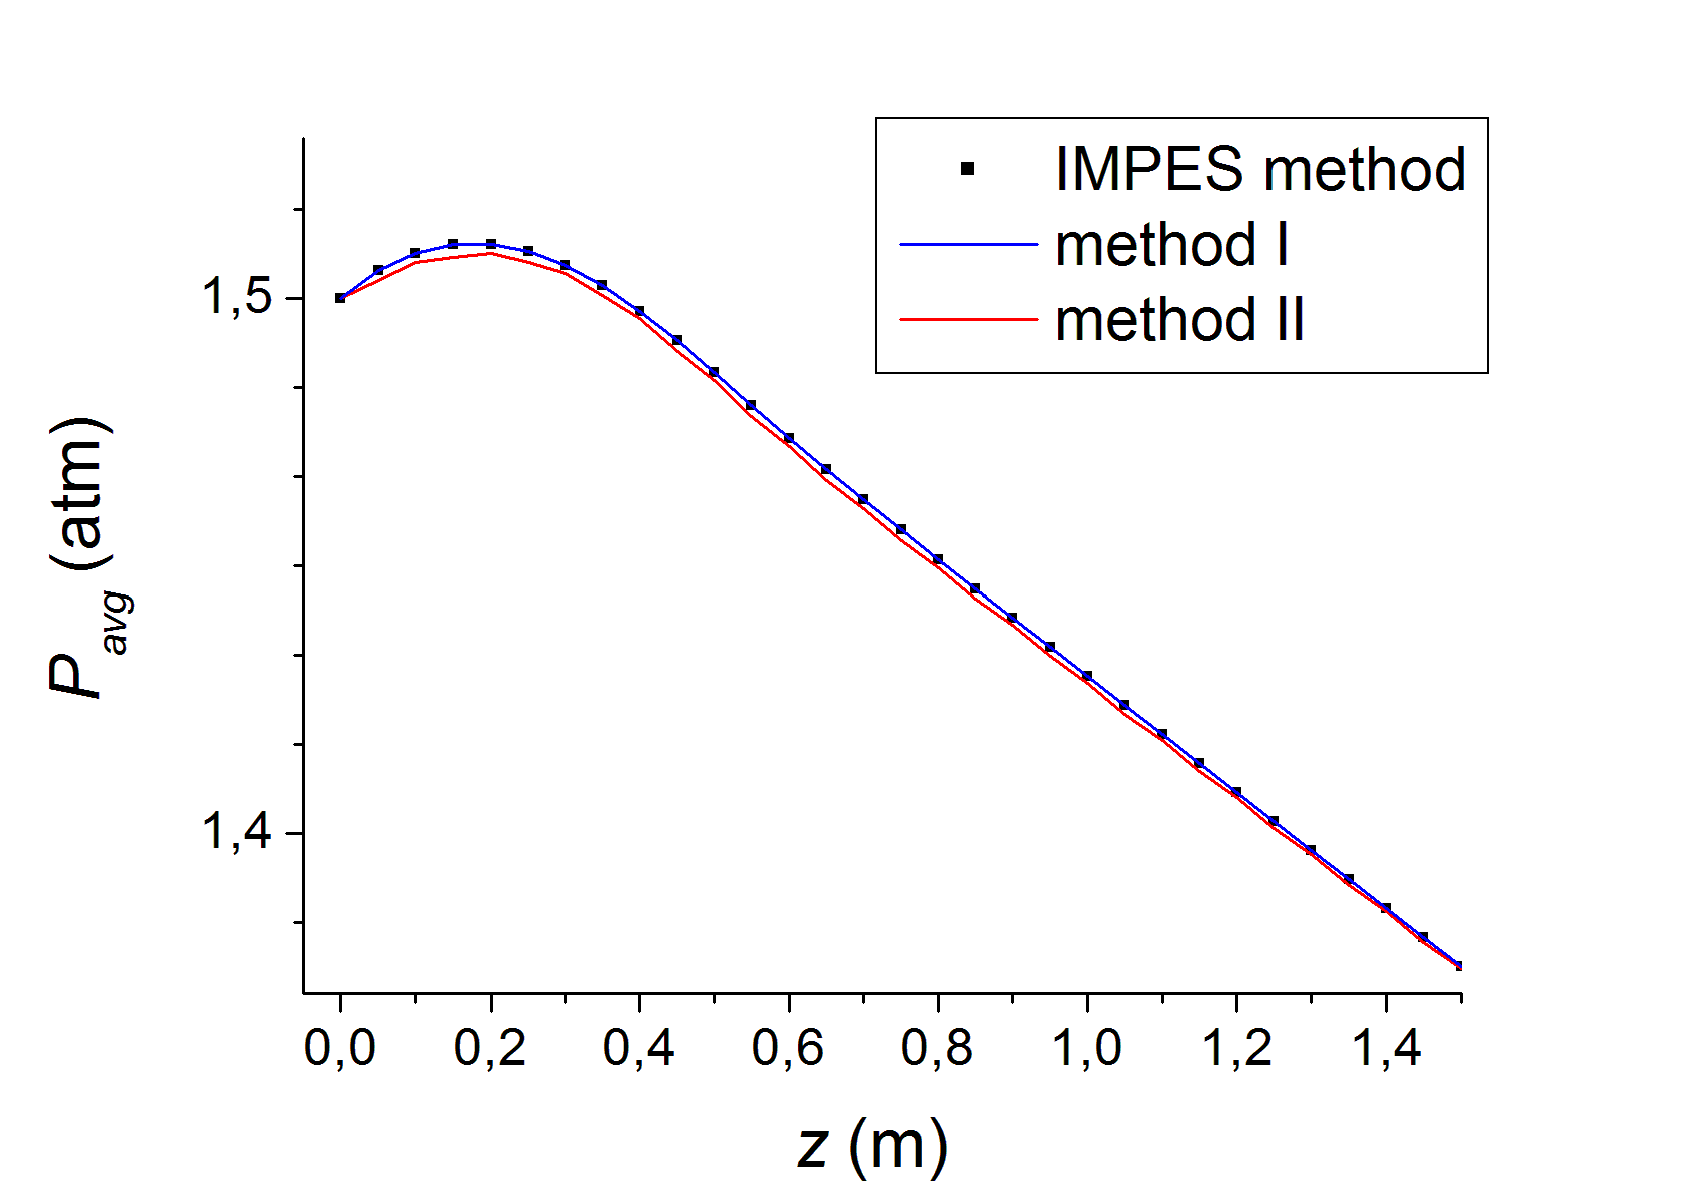
\includegraphics[width=1\textwidth]{test1/res2.png}
       \caption*{Среднее давление}
    \end{minipage}
  \caption{Распределение водонасыщенности и среднего давления фаз по глубине в момент времени 300c}
  \label{t1_pic2}
\end{figure}

\section{Сравнительный анализ алгоритмов явного типа} \label{ch:ch3/sect2}

Сравним устойчивость двух методов на примере задачи~\ref{ch:ch3/sect1}.
В таблице~\ref{tabular:limits} представлены максимально допустимые для устойчивости временные шаги, экспериментально полученные во время реализации методов I и II. 

\begin{table}[!ht]
\captionof{table}{Максимальные шаги по времени в алгоритмах на основе гиперболизированных уравнений}
\centering
\begin{tabular}{|c|c|c|}
\hline
\textit {h},м & $\Delta t$,с (метод I) & $\Delta t$,с (метод II) \\
\hline
0.05 & $1.5\cdot10^{-3}$ & $3\cdot10^{-4}$ \\
\hline
\end{tabular}
\label{tabular:limits}
\end{table}

Для метода I шаг подбирался таким образом, чтобы определитель при обращении матрицы в методе
Ньютона не становился равным нулю. Для метода II шаг выбирался из
условия критического нарастания ошибок, при котором решение <<разваливается>>.
В обоих случаях $\tau=\Delta t$ , то есть значение $\tau$ разное для методов I и II. Варьирование $\tau$ позволяет добиться
повышения $\Delta t$ еще в несколько раз, но не более.
В~\ref{tabular:limits} указан шаг
по времени для метода I больше в несколько раз, чем шаг для метода II, однако
метод I содержит реализацию метода Ньютона в каждом расчетном узле дополнительно по сравнению с явной схемой. По этой причине методы в целом сопоставимыми по вычислительным затратам.

В результате расчетов по методу II было установлено, что учет капиллярного
давления создает необходимость уменьшения шага по времени на порядок. Это можно объяснить сложной зависимостью уравнений для давления и насыщенности от преобладания тех или иных членов, например, при
доминировании капиллярных эффектов поведение решения становится типичным для
параболических уравнений, а ограничение на шаг по времени становится более жестким.

\section{Трехмерная трехфазная задача просачивания} \label{ch:ch3/sect3}

Исследуемая трехмерная область пористой среды -- куб размера
$\text{1м} \times \text{1м} \times \text{1м}$.
Верхняя грань открыта, нижняя -- ограничена резервуаром, через боковые грани
возможно просачивание.
Начальная постановка: вода занимает 10\% области,
нефть и газ распределены по периодическому закону. Ось $y$ направлена вертикально снизу-вверх.
В углу верхней грани расположен источник воды, который занимает девятую часть поверхности. Просачивание происходит под действием силы тяжести. 
Пусть число расчетных узлов -- $N_x\cdot N_y\cdot N_z$.\\
Начальные условия:
\begin{equation}
  \begin{aligned}
    &S_w=0.1,\\
    &S_n(x, y, z)=0.4 + 0.1 \cdot sin^2(x \cdot N_x + y \cdot N_y + z \cdot N_z),\\
    &S_g(x, y, z)=0.4 + 0.1 \cdot cos^2(x \cdot N_x + y \cdot N_y + z \cdot N_z),\\
    &P_w=P_\text{атм}.
   \end{aligned}
\end{equation}
Граничные условия:
\begin{equation}
  \begin{aligned}
    &\left.P\right|_{y=1,\ 0 < x < 0.33,\ 0 < z < 0.33}=P_{\text{атм}},\\
    &\left.{P_i}\right|_{y=0}\text{ определяется из условия } \left.(\overrightarrow{u_i} \cdot \overrightarrow{n})\right|_{y=0}=0;\\
    &\left.S_w\right|_{y=1,\ 0 < x < 0.33,\ 0 < z < 0.33}=0.6,\\
    &\left.S_n\right|_{y=1,\ 0 < x < 0.33,\ 0 < z < 0.33}=0.05,\\
    &\text{на остальных граничных поверхностях потоки}\\
    &S_w,\ S_n,\ P_w\ \text{эквиваленты нулю по направлению нормали.}
  \end{aligned}
\end{equation}

На ~\ref{t4_pic_start}-~\ref{t4_pic_end} проиллюстрированы результаты вычислений, приведены распределения давления,
и~насыщенностей водной и нефтяной фаз в три различные момента времени. Видно распространение фронтов от источника по области, вблизи нижней границы вода накопливается и постепенно вытесняет другие фазы через верхнюю и боковые грани.

\begin{figure}
\centering
    \begin{minipage}[!ht]{0.49\textwidth}
       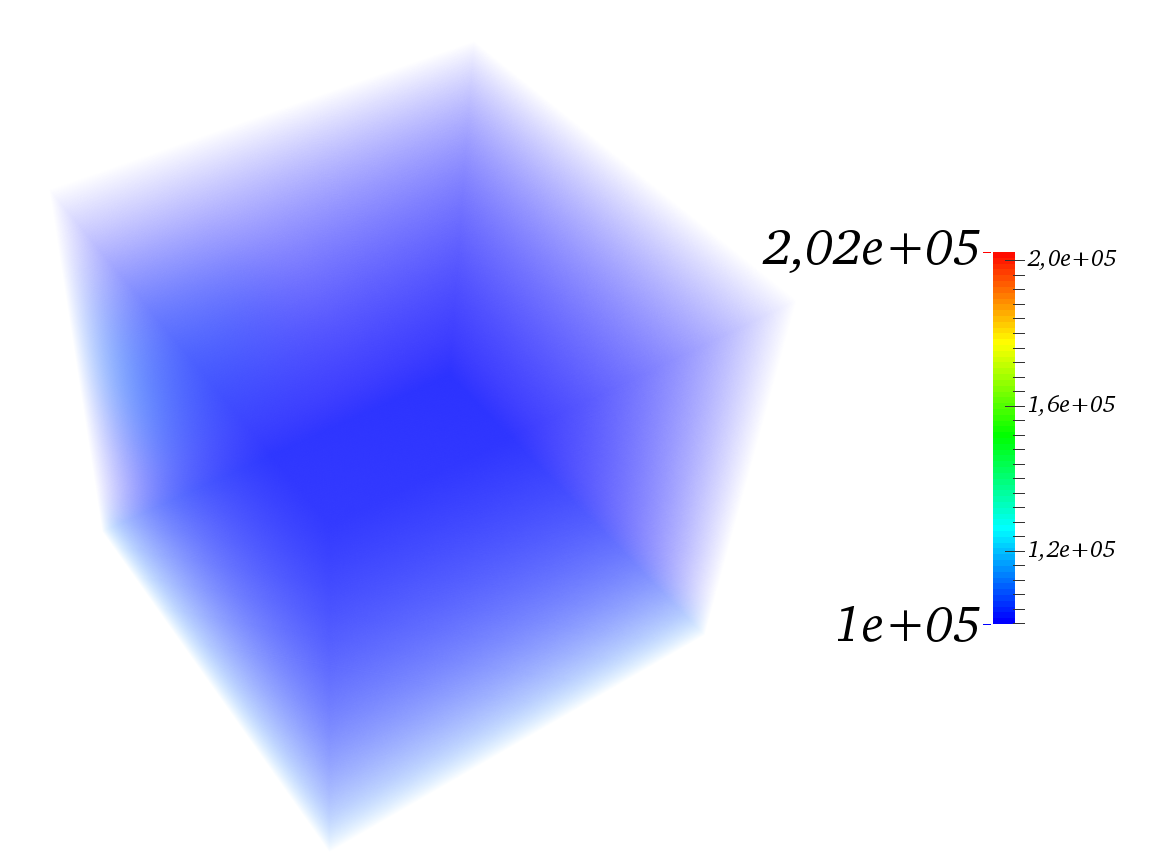
\includegraphics[width=1\textwidth]{test4/pw_200.png}
       \vspace{1cm}
       \caption{Давление $P_w$ в момент времени $t=200$с}
       \label{t4_pic_start}
    \end{minipage}
    \hfill
    \begin{minipage}[!ht]{0.49\textwidth}
       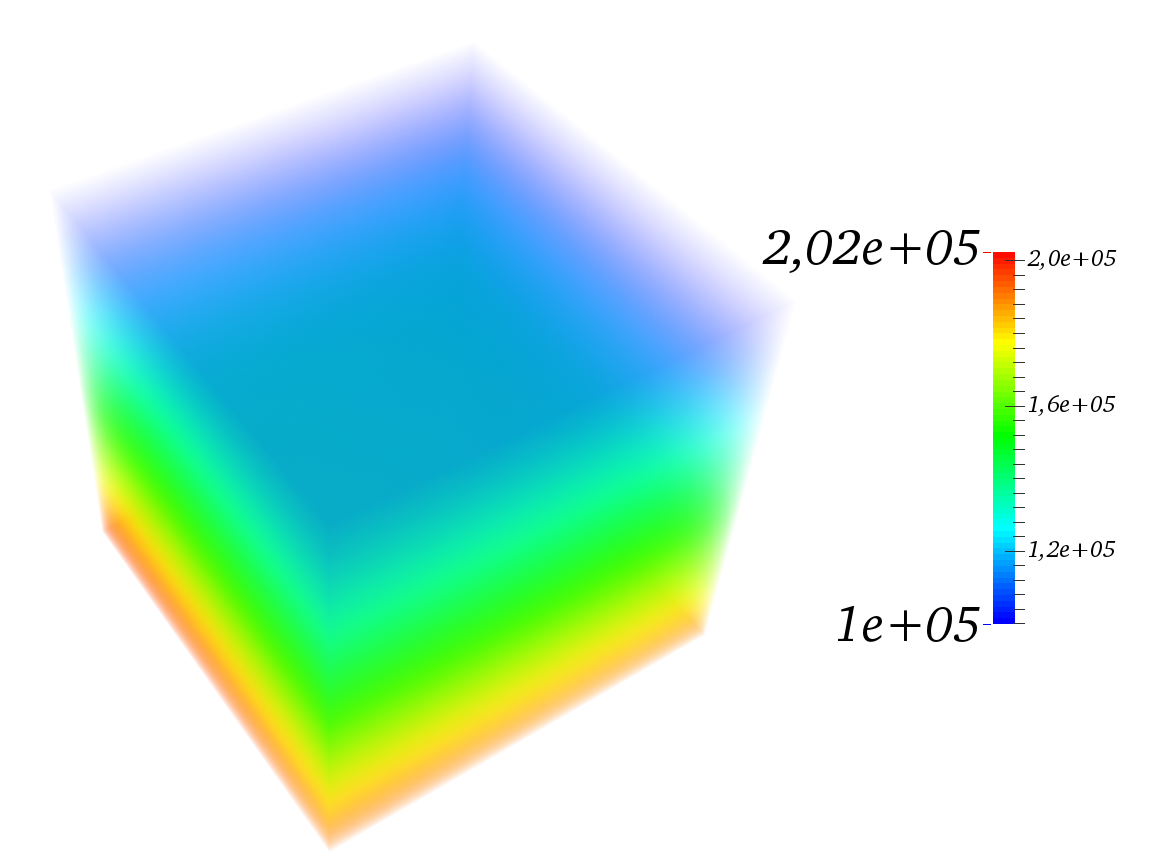
\includegraphics[width=1\textwidth]{test4/pw_1000.png}
       \vspace{1cm}
       \caption{Давление $P_w$ в момент времени $t=1000$с}
    \end{minipage}
    \vspace{3cm}
    \vfill
    \begin{minipage}[!ht]{0.49\textwidth}
       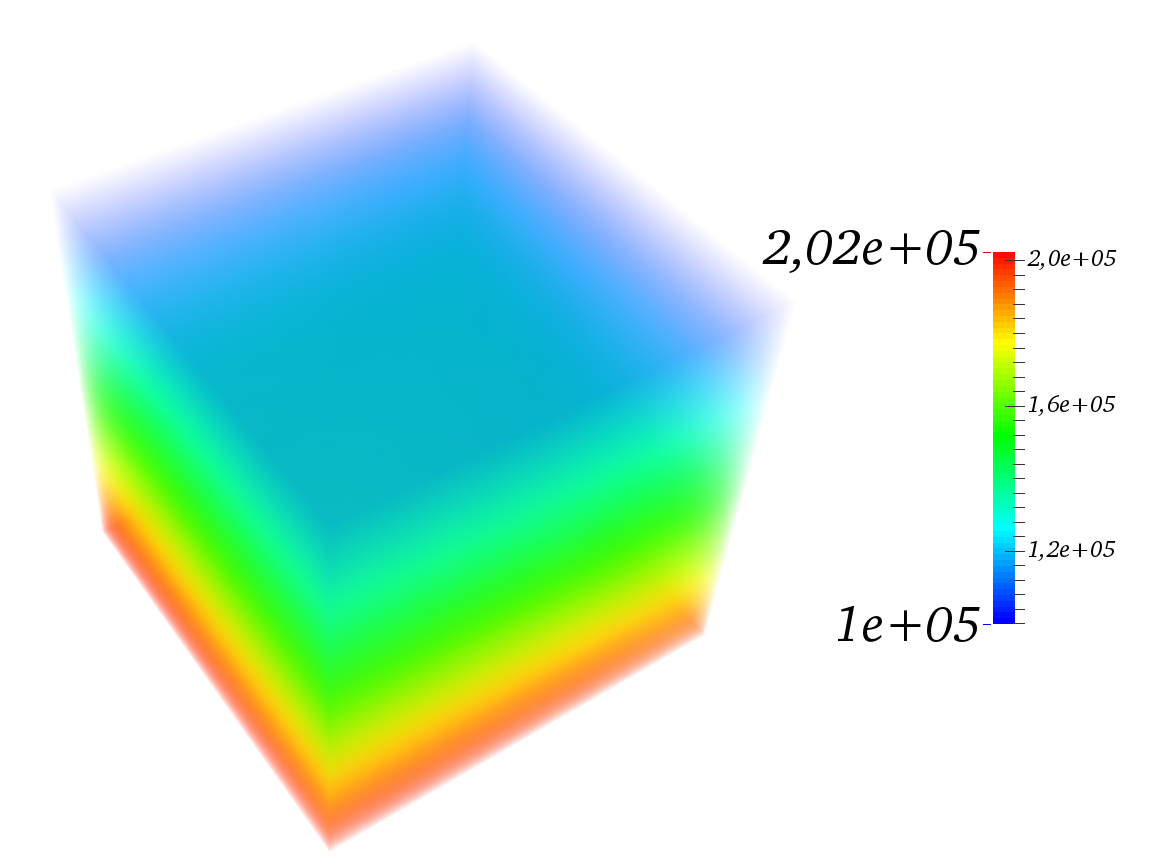
\includegraphics[width=1\textwidth]{test4/pw_2000.png}
       \vspace{1cm}
       \caption{Давление $P_w$ в момент времени $t=2000$с}
    \end{minipage}
    \hfill
    \begin{minipage}[!ht]{0.49\textwidth}
       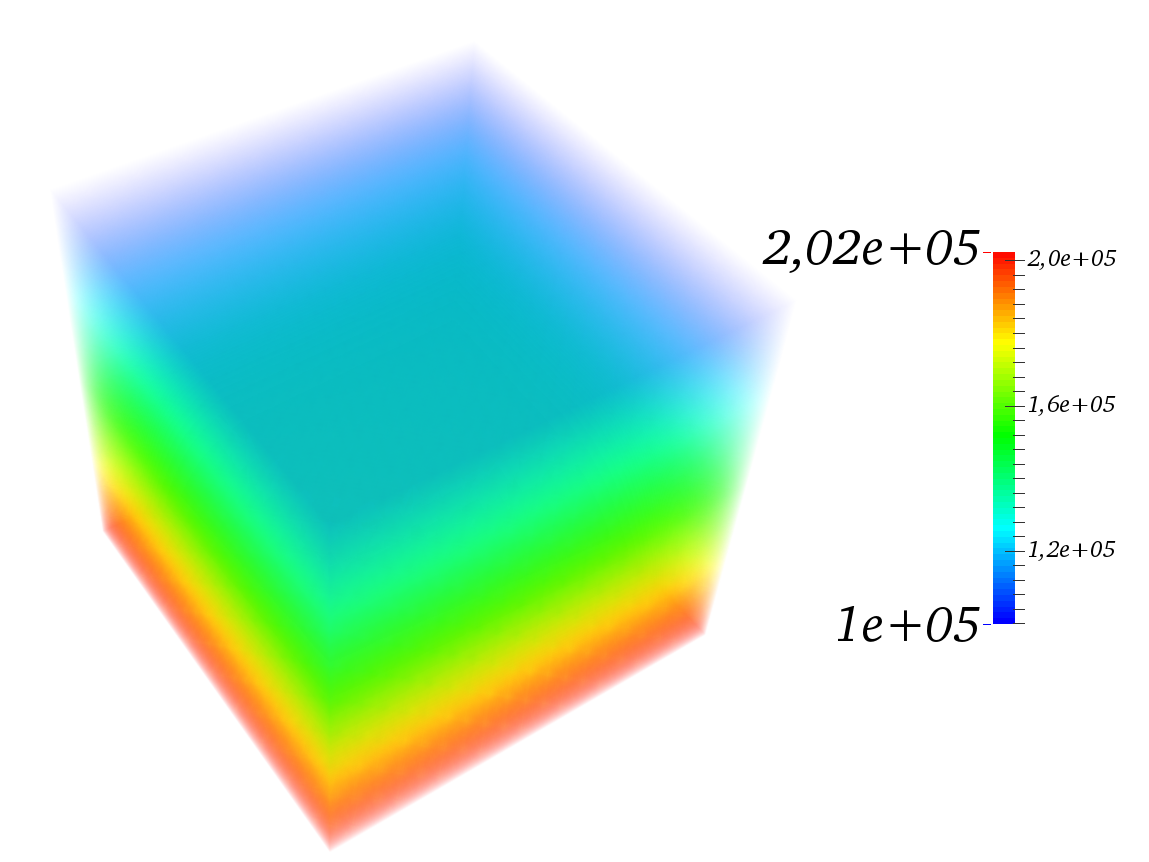
\includegraphics[width=1\textwidth]{test4/pw_6600.png}
       \vspace{1cm}
       \caption{Давление $P_w$ в момент времени $t=6600$с}
    \end{minipage}
    \hfill
\end{figure}

\begin{figure}
\centering
    \begin{minipage}[!ht]{0.49\textwidth}
       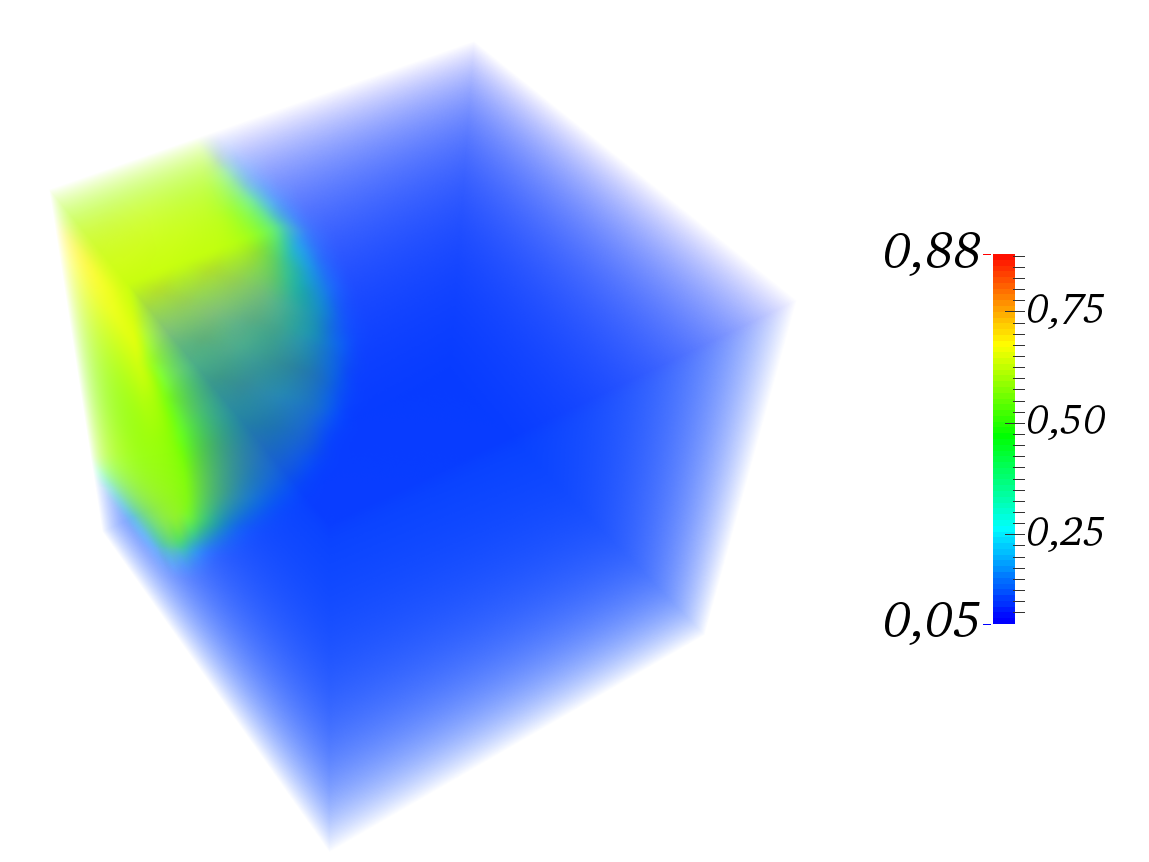
\includegraphics[width=1\textwidth]{test4/sw_200.png}
       \vspace{1cm}
       \caption{Насыщенность $S_w$ в момент времени $t=200$с}
    \end{minipage}
    \hfill
    \begin{minipage}[!ht]{0.49\textwidth}
       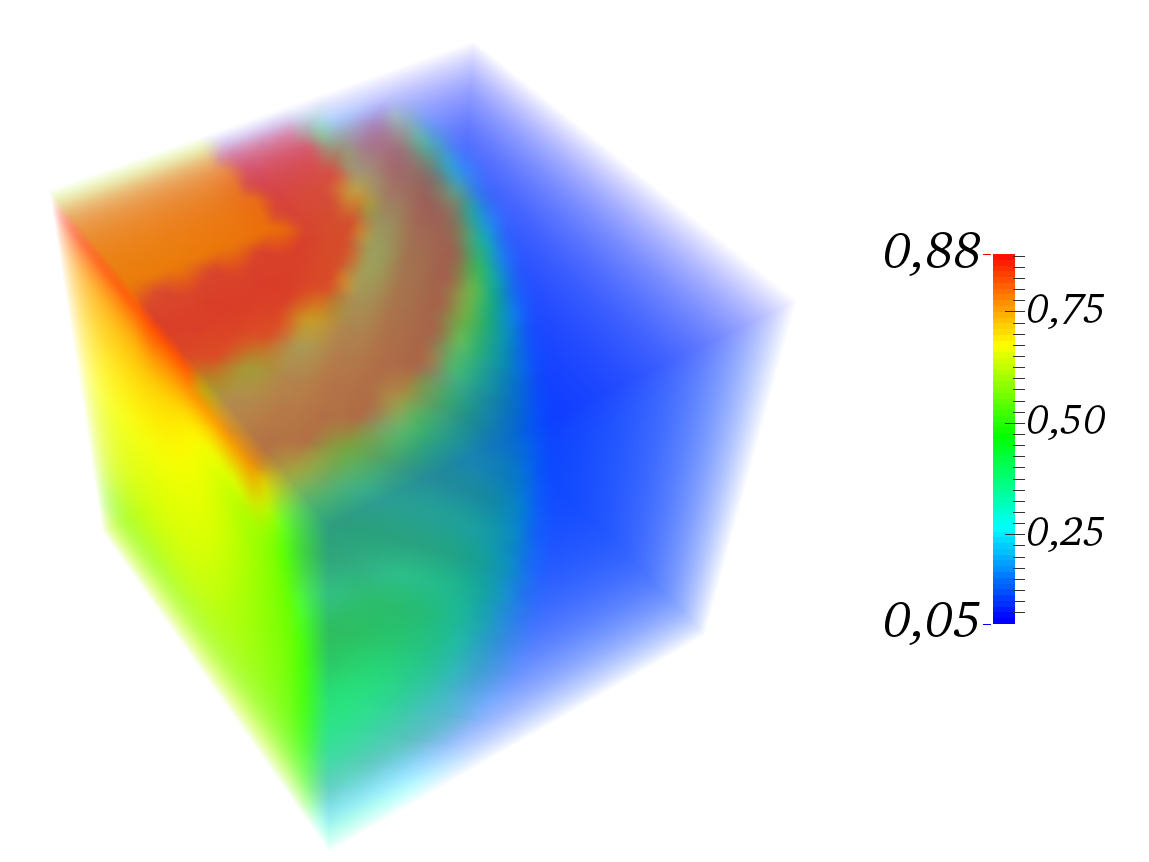
\includegraphics[width=1\textwidth]{test4/sw_1000.png}
       \vspace{1cm}
       \caption{Насыщенность $S_w$ в момент времени $t=1000$с}
    \end{minipage}
    \vspace{3cm}
    \vfill
    \begin{minipage}[!ht]{0.49\textwidth}
       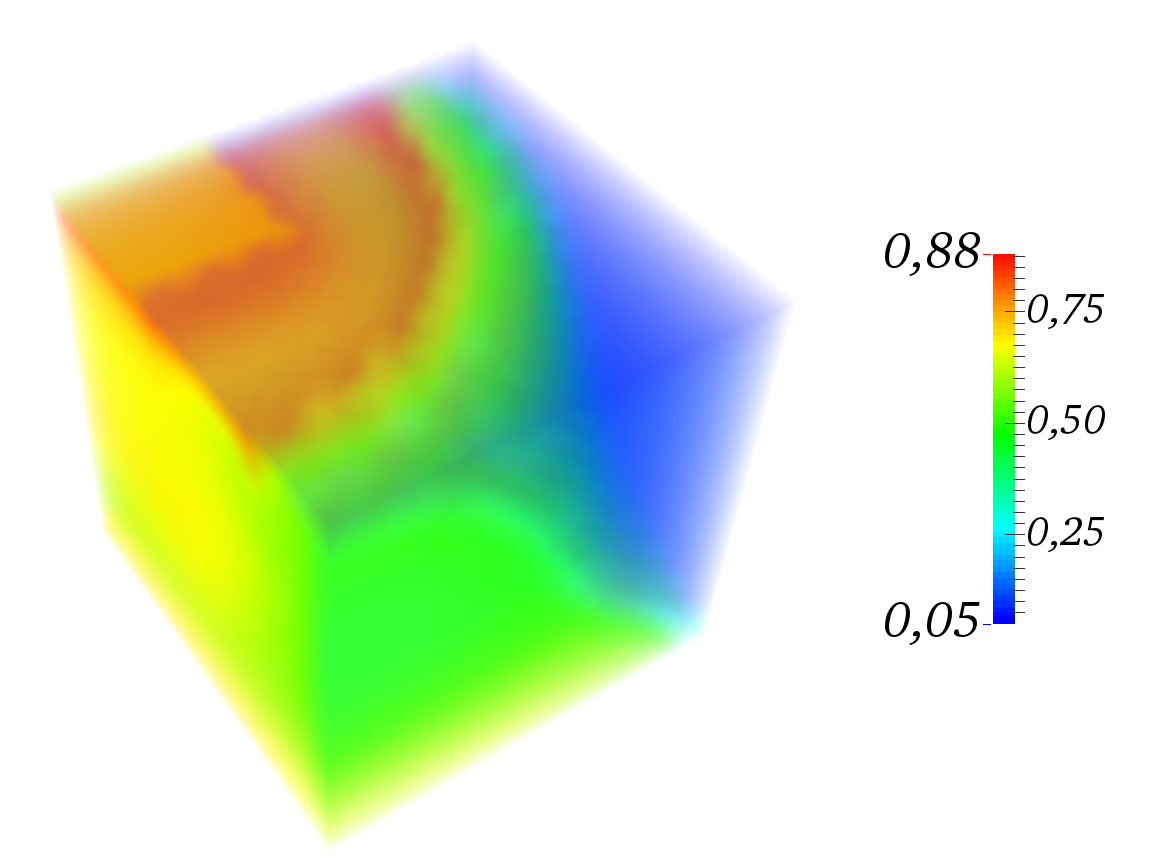
\includegraphics[width=1\textwidth]{test4/sw_2000.png}
       \vspace{1cm}
       \caption{Насыщенность $S_w$ в момент времени $t=2000$с}
    \end{minipage}
    \hfill
    \begin{minipage}[!ht]{0.49\textwidth}
       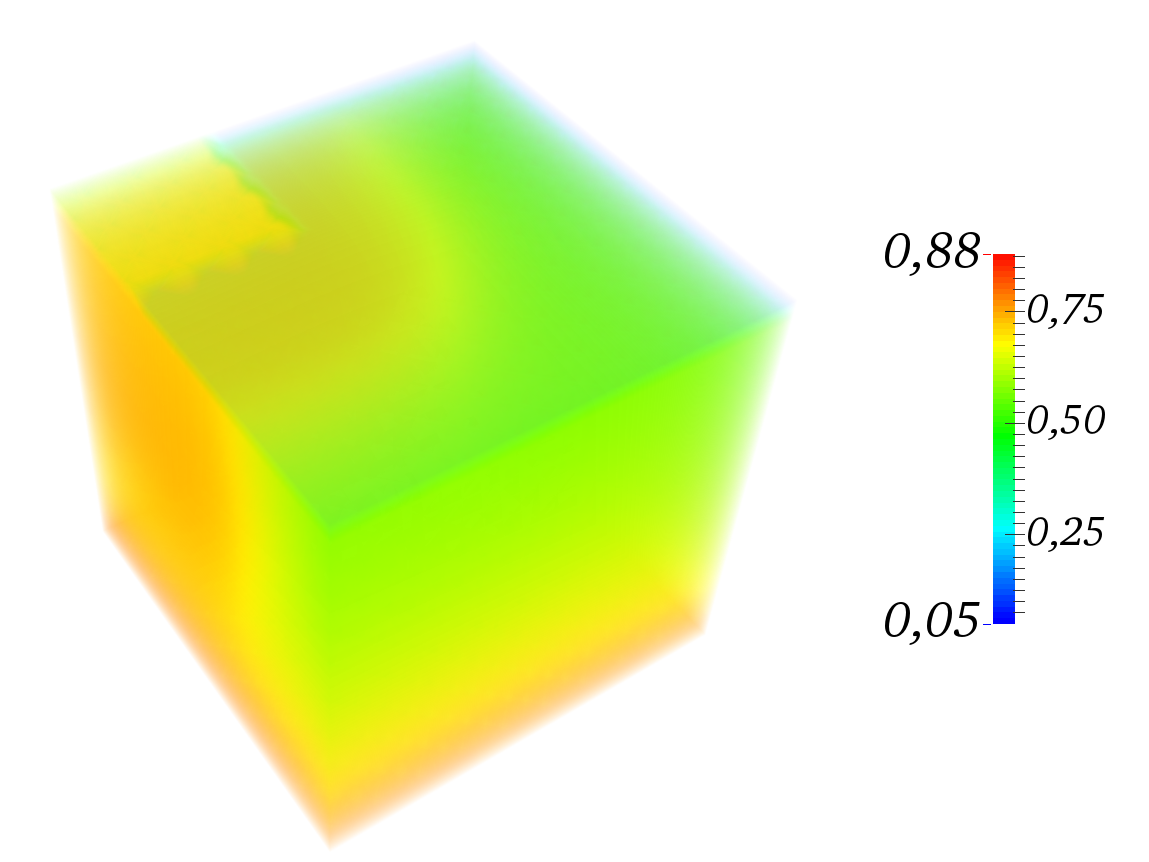
\includegraphics[width=1\textwidth]{test4/sw_6600.png}
       \vspace{1cm}
       \caption{Насыщенность $S_w$ в момент времени $t=6600$с}
    \end{minipage}
    \hfill
\end{figure}

\begin{figure}
\centering
    \begin{minipage}[!ht]{0.49\textwidth}
       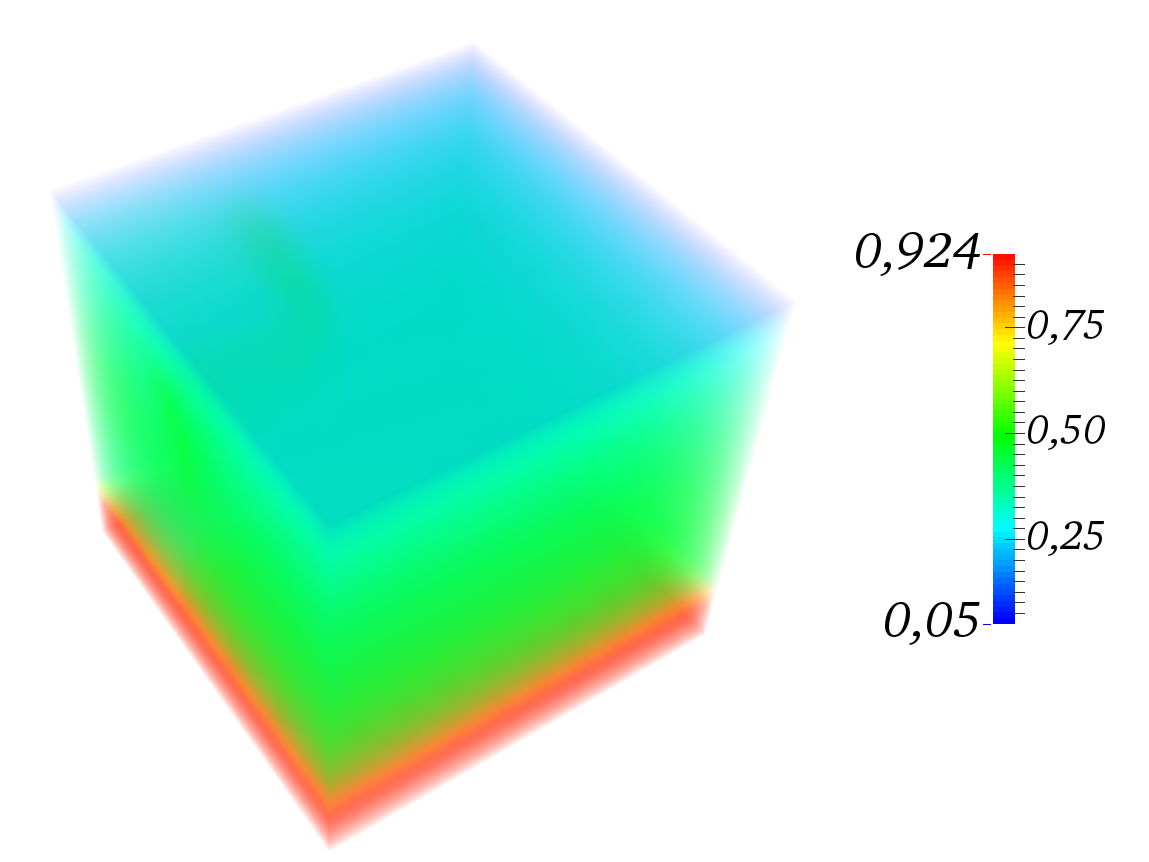
\includegraphics[width=1\textwidth]{test4/sn_200.png}
       \vspace{1cm}
       \caption{Насыщенность $S_n$ в момент времени $t=200$с}
    \end{minipage}
    \hfill
    \begin{minipage}[!ht]{0.49\textwidth}
       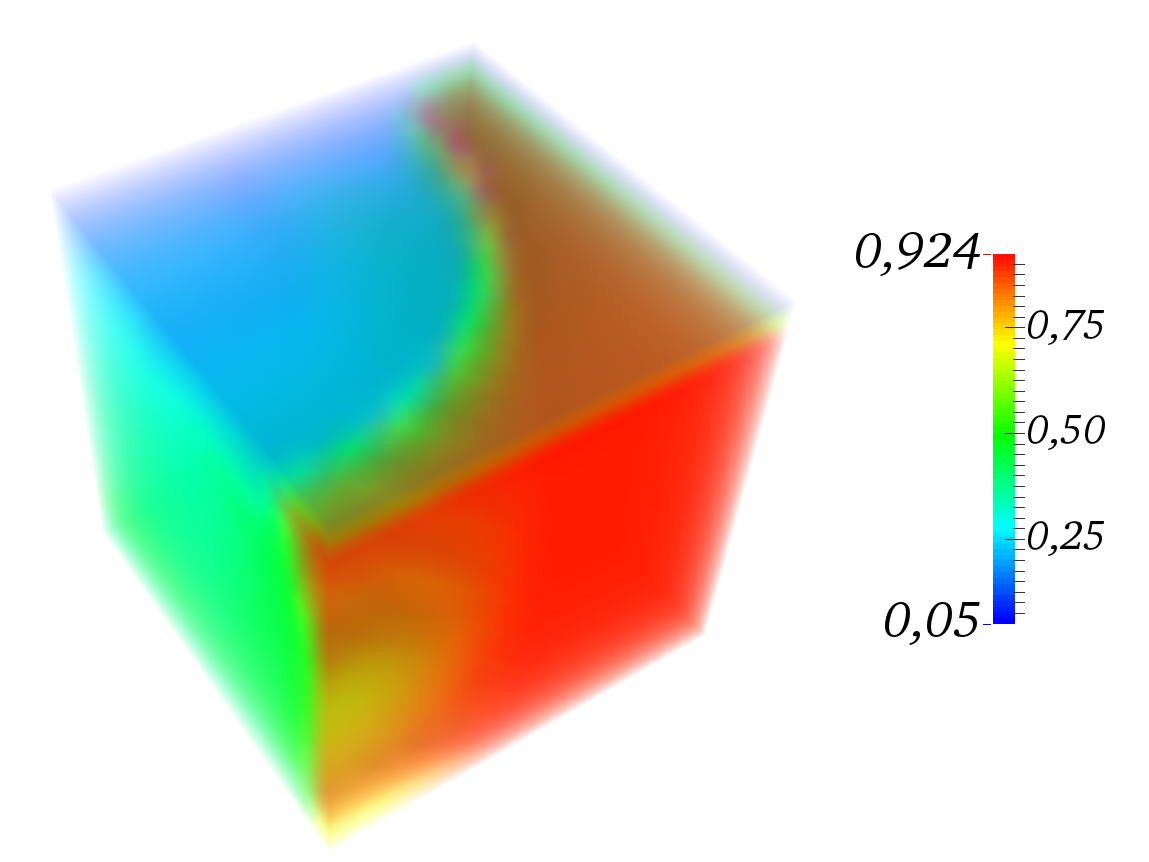
\includegraphics[width=1\textwidth]{test4/sn_1000.png}
       \vspace{1cm}
       \caption{Насыщенность $S_n$ в момент времени $t=1000$с}
    \end{minipage}
    \vspace{3cm}
    \vfill
    \begin{minipage}[!ht]{0.49\textwidth}
       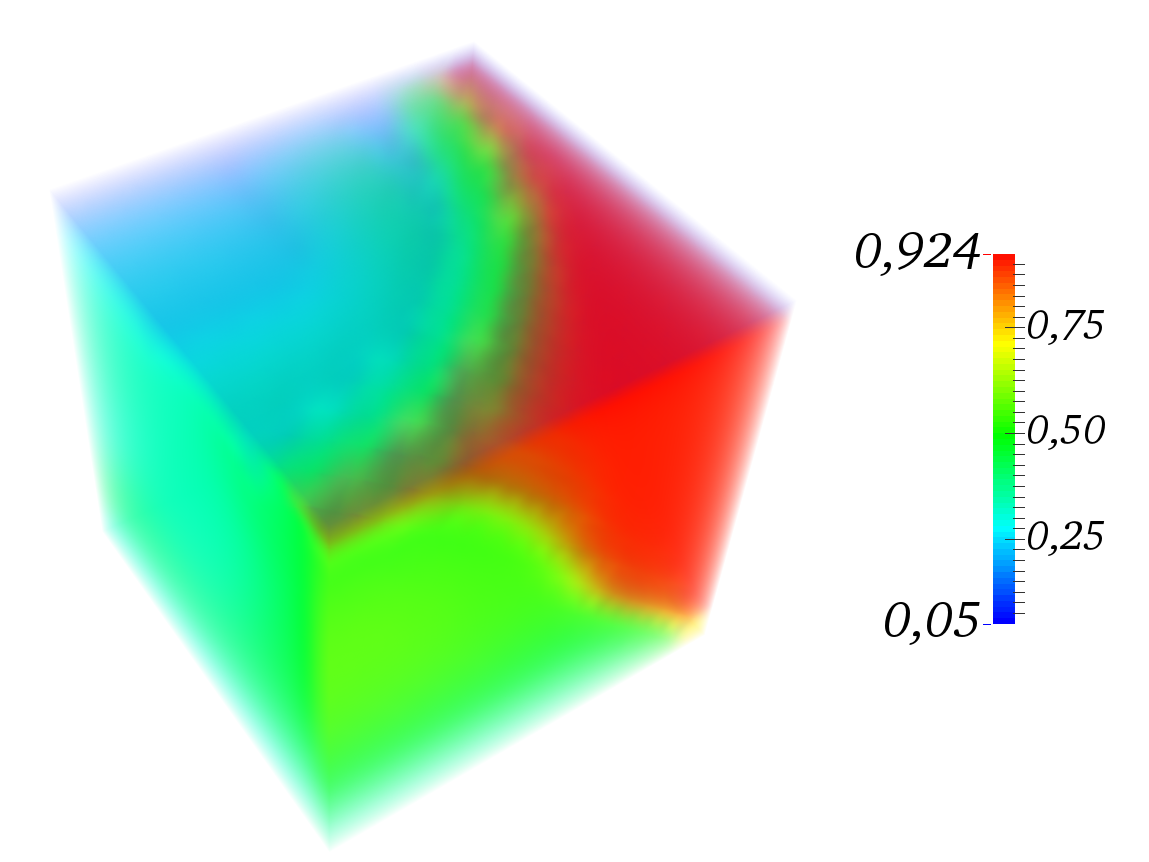
\includegraphics[width=1\textwidth]{test4/sn_2000.png}
       \vspace{1cm}
       \caption{Насыщенность $S_n$ в момент времени $t=2000$с}
    \end{minipage}
    \hfill
    \begin{minipage}[!ht]{0.49\textwidth}
       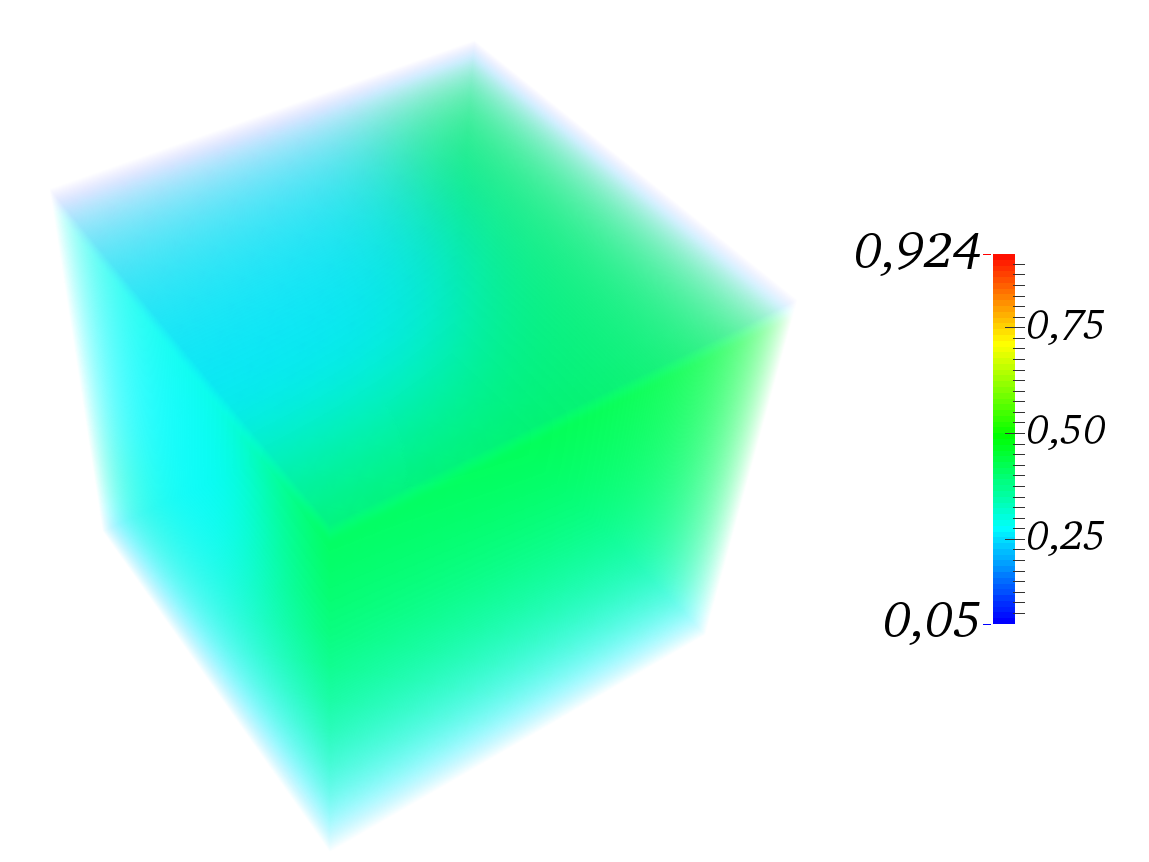
\includegraphics[width=1\textwidth]{test4/sn_6600.png}
       \vspace{1cm}
       \caption{Насыщенность $S_n$ в момент времени $t=6600$с}
       \label{t4_pic_end}
    \end{minipage}
    \hfill  
\end{figure}
